\begin{figure}[H]
    \centering
    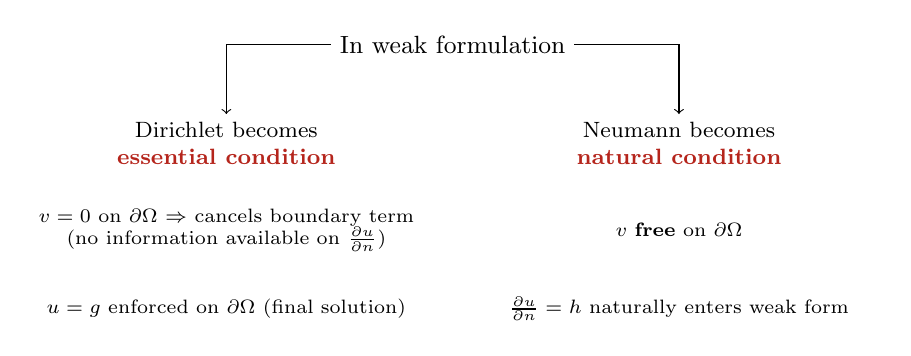
\begin{tikzpicture}
        \small

        \node at (0,5) (A) {In weak formulation};

        \footnotesize

        \node[align=center] at (-2.874,3.75) (B) {Dirichlet becomes\\ \textbf{\textcolor{BrickRed}{essential condition}}};
        \node[align=center] at (2.874,3.75) (C) {Neumann becomes\\ \textbf{\textcolor{BrickRed}{natural condition}}};

        \scriptsize

        \node[align=center,text width=4.86cm] at (-2.874,2.65) (D) {$\boldsymbol{v=0}$ on $\partial\Omega$ $\Rightarrow$ cancels boundary term\\ (no information available on $\frac{\partial u}{\partial n}$)};

        \node[align=center,text width=4.86cm] at (-2.874,1.65) (E) {$\boldsymbol{u=g}$ enforced on $\partial\Omega$ (final solution)};

        \node[align=center,text width=5cm] at (2.874,2.65) (F) {$\boldsymbol{v}$ \textbf{free} on $\partial\Omega$};

        \node[align=center,text width=5cm] at (2.874,1.65) (G) {$\boldsymbol{\frac{\partial u}{\partial n}=h}$ naturally enters weak form};

        \draw[->] (A) -- (-2.874,5) -- (B);
        \draw[->] (A) -- (2.874,5) -- (C);

        \normalsize
    \end{tikzpicture}
\end{figure}